\documentclass[../physics12.tex]{subfiles}
\graphicspath{{\subfix{../figures/}}}
\begin{document}
\chapter{Quantum Physics}
\section{Formulas for Chapters 15 and 16}
Mass-energy equivalence: $E=\gamma mc^2 = \sqrt{p^2c^2+m^2c^4}$

Lorentz factor: $\gamma = \sqrt{1-v^2/c^2}$

Photon energy: $E=hf-hc\lambda$

Photon momentum: $p=E/c$

Photoelectric effect: $KE_{\text{max}} = hf-\phi$

de Broglie wavelength: $\lambda = h/p$

Heisenberg's uncertainty principle: $\Delta x\Delta p_x \geq \frac{h}{4\pi}, \Delta E\Delta t \geq \frac{h}{4\pi}$

Bohr angular momentum quantization: 
\[ L = mvr_n = n\frac{h}{2\pi} (n=0,1,2,3,\dots) \]

Energy levels in hydrogen: $E_n = -13.6$ eV/n$^2$

Hydrogen spectrum wavelengths: $\frac{1}{\lambda} = R\{\frac{1}{n_f^2}-\frac{1}{n_i^2}\}$

Quantum numbers in atoms:

Principal quantum number: $n=1,2,3,\dots$

Orbital angular momentum:

mag: $L=\sqrt{l(l+1)}\cdot \frac{h}{2\pi} (l=0,1,\dots,n-1)$

z component: $L_z = \frac{m_l h}{2\pi} (m_l = -l,\dots,0,\dots l)$

Spin angular momentum:

mag: $S=\sqrt{s(s+1)}\cdot \frac{h}{2\pi} (s=\frac{1}{2}$ for electrons)

z component: $S_z = \frac{m_s h}{2\pi} (m_s = \pm \frac{1}{2})$

Mass number A, atomic number Z, and number of neutrons N: A = N + Z 

Size of nucleus: $r = r_0 A^{1/3}$, where $r_0$ = 1.2 fm 

Radioactive decay: $N=N_0e^{-\lambda t}=N_0 2^{-t/t_{1/2}}$ where $t_{1/2} = \ln 2/\lambda$

Decay rate: $R = \Delta N/\Delta t = 0.0693$N/$t_{1/2}$

Binding energy: BE = $\{[Zm(^1 H)+Nm_n]-m(^A X)\}c^2$

\section{Pulsed Laser Problem}
A vertical pulsed laster fires a 1000 MW pulse of 200 ns duration at a small 10 mg pellet at rest. The pulse hits the mass squarely in the center of its bottom side.
The speed of light is $3\times 10^8$ m/s and the acceleration of gravity is 9.8 m/s$^2$.
\begin{center}
    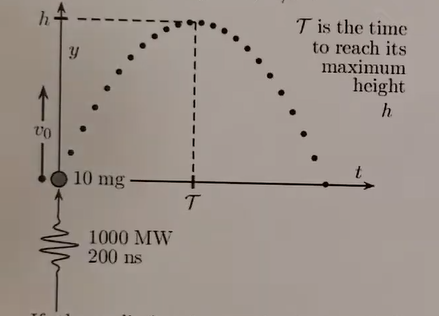
\includegraphics[width=0.5\textwidth]{15.1.PNG}
\end{center}
If the radiation is completely absorbed without other effects, what is the maximum height the mass reaches? Answer in units of $\mu$m.

\section{Solar Radiation Problem}
Solar radiation falls on Earth's surface at a rate of 1400 W/m$^2$.

ASsuming that the radiation has an average wavelength of 550 nm, how many photons per square meter per second fall on the surfaces? The speed of light is $3\times 10^8$ m/s and 
Planck's constant is $6.62607\times 10^{-34}$ J$\cdot$s. Answer in units of photons/m$^2\cdot$s.

\section{Electron Beam Diffraction Problem}
A beam of electrons, each with the same kinetic energy, illuminates a pair of slits separated by a distance of 54 nm. The beam forms bright and dark 
fringes on a screen located a distance 1.5 m beyond the two slits. The arrangement is otherwise identical to that used in the optical two-slit interference experiment. 
The bright fringes are found to be separated by a distance of 0.68 mm. 

What is the kinetic energy of the electrons in the beam? Planck's constant is $6.63\times 10^{-34}$ J$\cdot$s. Answer in units of keV.

\section{X-ray Tube Problem}
In the X-ray tube shown, a potential difference of 70000 V is applied across the two electrodes. Electrons emitted from the cathode are accelerated to the anode, where X-rays are produced.
\begin{center}
    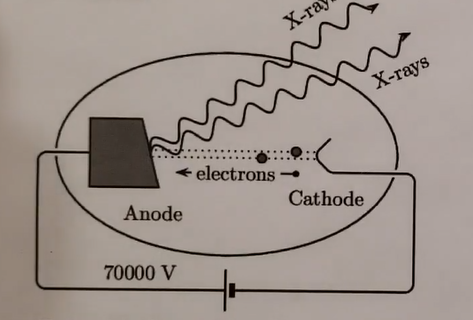
\includegraphics[width=0.5\textwidth]{15.2.PNG}
\end{center}
(a) Determine the maximum frequency of the X-rays produced by the tube. Answer in units of kHz.

(b) Find the maximum momentum of the X-ray photons produced by the tube. Answer in units of kg m/s.

\section{Alpha Particle and Gold Nucleus Problem}
(a) Find the speed of an alpha particle requires to come within $3.2\times 10^{-14}$ m of a gold nucleus. Coulomb's constant is $8.99\times 10^9$ N$\cdot$m$^2$/C$^2$, 
the charge on an electron is $1.6\times 10^{-19}$C, and the mass of the alpha particle is $6.64\times 10^{-27}$ kg. Answer in units of m/s.

(b) Find the energy of the alpha particle. Answer in units of MeV.

\section{Lyman Series Problem}
If, in 
\[ \frac{1}{\lambda} = R_y \left(\frac{1}{n_1^2}-\frac{1}{n_2^2}\right) \]
you set $n_1 = 1$ and take $n_2$ greater than 1, you generate what is known as the Lyman series.

(a) Find the wavelength of the first member of this series. The value of $\hbar$ is $1.05457\times 10^{-34}$ J$\cdot$s; the Rydberg constant for 
hydrogen is $1.09735\times 10^7$ m$^{-1}$; the Bohr radius is $5.29177\times 10^{-11}$ m; and the ground state energy for hydrogen is 13.6057 eV. Answer in units of nm.

(b) Consider the next three members of this series. The wavelengths of successive members of the Lyman series approach a common limit as $n_2 \rightarrow \infty$. What is this limit? Answer in units of nm.

\section{Bohr Model Problem}
Using the Bohr model, find the ionization energy of the ground He$^+$ ion. Answer in units of eV.

\section{Energy of Magnetic Moment Problem}
The potential energy of a magnetic moment in an external magnetic field is given by $U=-\mu\cdot\vec{B}$. The magnetic moment associated with the 
spin of an electron is $5.79\times 10^{-5}$ eV/T. 

(a) Calculate the difference in energy between the two possible orientations of an electron in energy in a magnetic field $\vec{B}=(0.6$T)$\hat{k}$. Answer in units of eV.

(b) If these electrons are bombarded with photos of energy equal to this energy difference, ``spin flip'' transitions can be induced. Find the wavelength 
of thie photons needed for such transitions. (This phenomenon is called electron spin resistance). Answer in units of cm.
\end{document}